% ===== 06-mle =====
\section*{Maximum Likelihood Estimation (MLE)}

\subsection*{Probability vs.\ Likelihood}
\textbf{Setup:} data $\mathcal{D} = \{x_1, \dots, x_N\}$ from a model $p(x \mid \theta)$, where $\theta$ = the model's parameters.

Running example: flip a coin $N = 10$ times and get $n_1 = 7$ heads. Here $\theta$ = probability of heads.

\begin{itemize}
  \item \textbf{Probability:} $\theta$ is fixed, and we ask how likely the data is.\\
  Fair coin ($\theta = 0.5$): $P(\text{7 heads in 10} \mid \theta = 0.5) = \binom{10}{7}(0.5)^7(0.5)^3 \approx 0.117$.
  \item \textbf{Likelihood:} the data is fixed, and we ask how well each $\theta$ explains it.\\
  After seeing 7 heads: $L(0.7) \approx 0.267$ beats $L(0.5) \approx 0.117$.
\end{itemize}
\[
L(\theta) = p(\mathcal{D} \mid \theta)
\qquad \text{coin:} \quad L(\theta) = \binom{10}{7}\,\theta^7 (1-\theta)^3
\]

Same formula, different variable: probability varies the data, likelihood varies $\theta$.

\begin{keeptogether}
{\centering
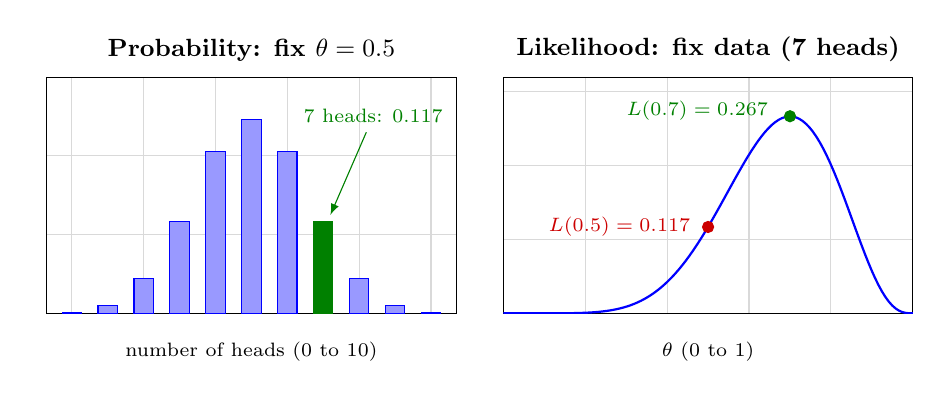
\begin{tikzpicture}
% ---- probability: vary the data ----
\begin{axis}[name=prob, scale only axis, width=5.2cm, height=3cm,
    xmin=-0.7, xmax=10.7, ymin=0, ymax=0.3, enlargelimits=false,
    grid=major, grid style={gray!30}, major tick length=0pt,
    xticklabels={}, yticklabels={},
    title={\small\textbf{Probability: fix $\theta = 0.5$}}, title style={yshift=-4pt},
    xlabel={\scriptsize number of heads (0 to 10)}, label style={font=\scriptsize}]
\addplot[ybar, bar shift=0pt, bar width=7pt, fill=blue!40, draw=blue] coordinates {
  (0,0.001) (1,0.010) (2,0.044) (3,0.117) (4,0.205) (5,0.246)
  (6,0.205) (8,0.044) (9,0.010) (10,0.001)};
\addplot[ybar, bar shift=0pt, bar width=7pt, fill=green!50!black, draw=green!50!black] coordinates {(7,0.117)};
\node[font=\scriptsize, green!50!black, anchor=south east] at (axis cs:10.6,0.23) {7 heads: 0.117};
\addplot[green!50!black, -latex] coordinates {(8.2,0.23) (7.2,0.125)};
\end{axis}
% ---- likelihood: vary theta ----
\begin{axis}[name=lik, at={(prob.east)}, anchor=west, xshift=0.6cm,
    scale only axis, width=5.2cm, height=3cm,
    xmin=0, xmax=1, ymin=0, ymax=0.32, enlargelimits=false,
    grid=major, grid style={gray!30}, major tick length=0pt,
    xticklabels={}, yticklabels={},
    title={\small\textbf{Likelihood: fix data (7 heads)}}, title style={yshift=-4pt},
    xlabel={\scriptsize $\theta$ (0 to 1)}, label style={font=\scriptsize}]
\addplot[thick, blue, domain=0:1, samples=120] {120*x^7*(1-x)^3};
\addplot[only marks, mark=*, red!80!black, mark size=2pt] coordinates {(0.5,0.117)};
\node[font=\scriptsize, red!80!black, anchor=east] at (axis cs:0.48,0.117) {$L(0.5) = 0.117$};
\addplot[only marks, mark=*, green!50!black, mark size=2pt] coordinates {(0.7,0.267)};
\node[font=\scriptsize, green!50!black, anchor=east] at (axis cs:0.67,0.275) {$L(0.7) = 0.267$};
\end{axis}
\end{tikzpicture}
\par}
\end{keeptogether}

\subsection*{What MLE Does}
\textbf{MLE turns estimation into an optimization problem:} pick the parameter that maximizes the likelihood (the peak of the curve):
\[
\theta_{\text{ML}} = \arg\max_{\theta} L(\theta) = \arg\max_{\theta} \ln L(\theta) = \arg\min_{\theta} \big(-\ln L(\theta)\big)
\]

\textbf{Why log?} $\ln$ is monotonic, so the peak doesn't move. And it turns a product into a sum, which is much easier to differentiate:
\[
\tfrac{d}{d\theta}\big[\theta^7(1-\theta)^3\big] \;\text{(product rule, messy)}
\qquad \text{vs.} \qquad
\tfrac{d}{d\theta}\big[7\ln \theta + 3\ln(1-\theta)\big] = \tfrac{7}{\theta} - \tfrac{3}{1-\theta}
\]

\subsection*{Finding the Peak in 3 Steps}
\begin{keeptogether}
\textbf{Step 1: Independent \& Identically Distributed $\Rightarrow$ product.} Each data point $x_n$ is independent, so the likelihood multiplies:
\[
p(\mathcal{D} \mid \theta) = \prod_{n=1}^{N} p(x_n \mid \theta)
\]
Coin: each head contributes $\theta$ and each tail contributes $(1-\theta)$. With 7 heads and 3 tails:
\[
p(\mathcal{D} \mid \theta) = \underbrace{\theta \cdots \theta}_{7 \text{ heads}} \cdot \underbrace{(1-\theta) \cdots (1-\theta)}_{3 \text{ tails}} = \theta^{7}(1-\theta)^{3}
\]
\end{keeptogether}

\begin{keeptogether}
\textbf{Step 2: Log $\Rightarrow$ sum.} The log turns the product into a sum, and the peak stays in the same place:
\[
\ln p(\mathcal{D} \mid \theta) = \sum_{n=1}^{N} \ln p(x_n \mid \theta)
\qquad \text{coin:} \quad 7 \ln \theta + 3 \ln(1-\theta)
\]

{\centering
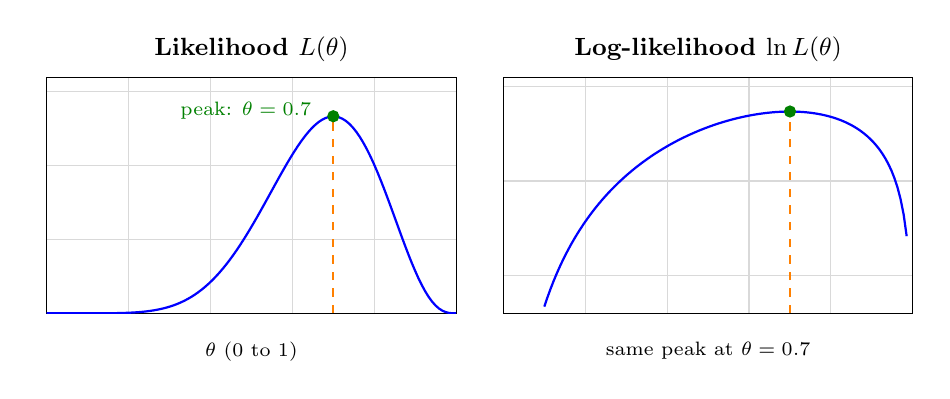
\begin{tikzpicture}
% ---- L(theta) ----
\begin{axis}[name=L, scale only axis, width=5.2cm, height=3cm,
    grid=major, grid style={gray!30}, major tick length=0pt,
    xticklabels={}, yticklabels={}, title style={yshift=-4pt}, label style={font=\scriptsize},
    xmin=0, xmax=1, ymin=0, ymax=0.32, enlargelimits=false,
    title={\small\textbf{Likelihood $L(\theta)$}},
    xlabel={\scriptsize $\theta$ (0 to 1)}]
\addplot[thick, blue, domain=0:1, samples=120] {120*x^7*(1-x)^3};
\addplot[orange, dashed, thick] coordinates {(0.7,0) (0.7,0.267)};
\addplot[only marks, mark=*, green!50!black, mark size=2pt] coordinates {(0.7,0.267)};
\node[font=\scriptsize, green!50!black, anchor=east] at (axis cs:0.67,0.275) {peak: $\theta = 0.7$};
\end{axis}
% ---- ln L(theta) ----
\begin{axis}[name=lnL, at={(L.east)}, anchor=west, xshift=0.6cm, scale only axis, width=5.2cm, height=3cm,
    grid=major, grid style={gray!30}, major tick length=0pt,
    xticklabels={}, yticklabels={}, title style={yshift=-4pt}, label style={font=\scriptsize},
    xmin=0, xmax=1, ymin=-12, ymax=0.5, enlargelimits=false,
    title={\small\textbf{Log-likelihood $\ln L(\theta)$}},
    xlabel={\scriptsize same peak at $\theta = 0.7$}]
\addplot[thick, blue, domain=0.1:0.985, samples=120] {ln(120) + 7*ln(x) + 3*ln(1-x)};
\addplot[orange, dashed, thick] coordinates {(0.7,-12) (0.7,-1.32)};
\addplot[only marks, mark=*, green!50!black, mark size=2pt] coordinates {(0.7,-1.32)};
\end{axis}
\end{tikzpicture}
\par}
\end{keeptogether}

\begin{keeptogether}
\textbf{Step 3: Maximize the likelihood.} Set the derivative to 0 and solve, since the slope is flat at the peak:
\[
\frac{\partial}{\partial \theta} \ln p(\mathcal{D} \mid \theta) = 0
\qquad \text{coin:} \quad \frac{7}{\theta} - \frac{3}{1-\theta} = 0
\;\Rightarrow\; 7(1-\theta) = 3\theta
\;\Rightarrow\; \theta_{\text{ML}} = \frac{7}{10}
\]
In general (Bernoulli): $\theta_{\text{ML}} = \frac{n_1}{N}$, the fraction of heads.

{\centering
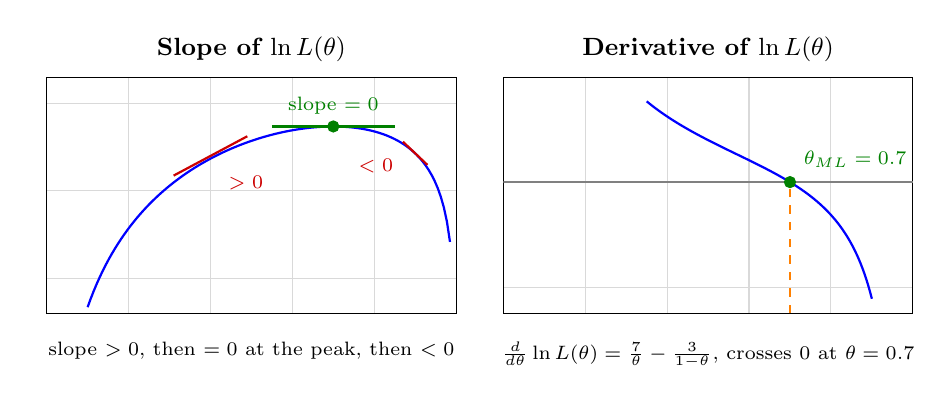
\begin{tikzpicture}
% ---- ln L with tangent lines ----
\begin{axis}[name=tan, scale only axis, width=5.2cm, height=3cm,
    grid=major, grid style={gray!30}, major tick length=0pt,
    xticklabels={}, yticklabels={}, title style={yshift=-4pt}, label style={font=\scriptsize},
    xmin=0, xmax=1, ymin=-12, ymax=1.5, enlargelimits=false,
    title={\small\textbf{Slope of $\ln L(\theta)$}},
    xlabel={\scriptsize slope $> 0$, then $= 0$ at the peak, then $< 0$}]
\addplot[thick, blue, domain=0.1:0.985, samples=120] {ln(120) + 7*ln(x) + 3*ln(1-x)};
\addplot[red!80!black, thick] coordinates {(0.31,-4.13) (0.49,-1.88)};
\node[font=\scriptsize, red!80!black, anchor=north west] at (axis cs:0.42,-3.6) {$> 0$};
\addplot[green!50!black, thick] coordinates {(0.55,-1.32) (0.85,-1.32)};
\node[font=\scriptsize, green!50!black, anchor=south] at (axis cs:0.7,-1.2) {slope $= 0$};
\addplot[red!80!black, thick] coordinates {(0.87,-2.19) (0.93,-3.52)};
\node[font=\scriptsize, red!80!black, anchor=east] at (axis cs:0.87,-3.6) {$< 0$};
\addplot[only marks, mark=*, green!50!black, mark size=2pt] coordinates {(0.7,-1.32)};
\end{axis}
% ---- derivative ----
\begin{axis}[name=der, at={(tan.east)}, anchor=west, xshift=0.6cm, scale only axis, width=5.2cm, height=3cm,
    grid=major, grid style={gray!30}, major tick length=0pt,
    xticklabels={}, yticklabels={}, title style={yshift=-4pt}, label style={font=\scriptsize},
    xmin=0, xmax=1, ymin=-25, ymax=20, enlargelimits=false,
    title={\small\textbf{Derivative of $\ln L(\theta)$}},
    xlabel={\scriptsize $\frac{d}{d\theta}\ln L(\theta) = \frac{7}{\theta} - \frac{3}{1-\theta}$, crosses 0 at $\theta = 0.7$}]
\addplot[gray, thick] coordinates {(0,0) (1,0)};
\addplot[thick, blue, domain=0.35:0.9, samples=120] {7/x - 3/(1-x)};
\addplot[orange, dashed, thick] coordinates {(0.7,-25) (0.7,0)};
\addplot[only marks, mark=*, green!50!black, mark size=2pt] coordinates {(0.7,0)};
\node[font=\scriptsize, green!50!black, anchor=south west] at (axis cs:0.71,1) {$\theta_{\text{ML}} = 0.7$};
\end{axis}
\end{tikzpicture}
\par}
\end{keeptogether}
\subsection*{MLE for Linear Regression}
\textbf{Two ways to fit a line:}

\begin{itemize}
    \item \textbf{Least squares:} pick the line with the smallest squared error $E(\mathbf{w}) = \frac{1}{2}\sum_n (t_n - \mathbf{w}^\top\mathbf{x}_n)^2$.
  \item \textbf{MLE:} pick the line that makes \emph{all} the points most likely, assuming Gaussian noise.
\end{itemize}

\textbf{Big idea: they give the same line.} Least squares is MLE with Gaussian noise. Here $\theta = \mathbf{w}$ (the line's weights, not a probability like in the coin example).

\begin{keeptogether}
{\centering
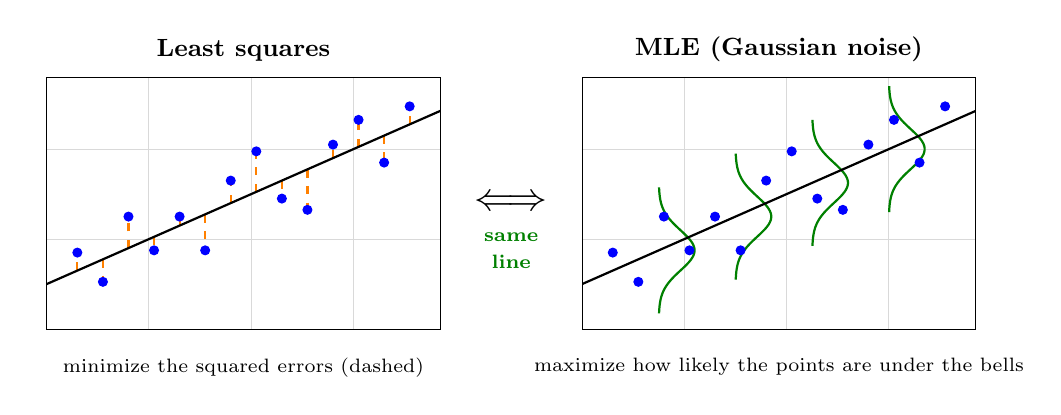
\begin{tikzpicture}
\begin{axis}[name=ls, scale only axis, width=5cm, height=3.2cm,
    xmin=0, xmax=7.7, ymin=0, ymax=5.6, enlargelimits=false, grid=major, grid style={gray!30}, major tick length=0pt,
    xticklabels={}, yticklabels={}, title style={yshift=-4pt}, label style={font=\scriptsize},
    title={\small\textbf{Least squares}},
    xlabel={\scriptsize minimize the squared errors (dashed)}]
\addplot[orange, dashed, thick] coordinates {(0.6,1.30) (0.6,1.7)};
\addplot[orange, dashed, thick] coordinates {(1.1,1.55) (1.1,1.05)};
\addplot[orange, dashed, thick] coordinates {(1.6,1.80) (1.6,2.5)};
\addplot[orange, dashed, thick] coordinates {(2.1,2.05) (2.1,1.75)};
\addplot[orange, dashed, thick] coordinates {(2.6,2.30) (2.6,2.5)};
\addplot[orange, dashed, thick] coordinates {(3.1,2.55) (3.1,1.75)};
\addplot[orange, dashed, thick] coordinates {(3.6,2.80) (3.6,3.3)};
\addplot[orange, dashed, thick] coordinates {(4.1,3.05) (4.1,3.95)};
\addplot[orange, dashed, thick] coordinates {(4.6,3.30) (4.6,2.9)};
\addplot[orange, dashed, thick] coordinates {(5.1,3.55) (5.1,2.65)};
\addplot[orange, dashed, thick] coordinates {(5.6,3.80) (5.6,4.1)};
\addplot[orange, dashed, thick] coordinates {(6.1,4.05) (6.1,4.65)};
\addplot[orange, dashed, thick] coordinates {(6.6,4.30) (6.6,3.7)};
\addplot[orange, dashed, thick] coordinates {(7.1,4.55) (7.1,4.95)};
\addplot[thick, black, domain=0:7.7] {1 + 0.5*x};
\addplot[only marks, mark=*, blue, mark size=1.6pt] coordinates {(0.6,1.7) (1.1,1.05) (1.6,2.5) (2.1,1.75) (2.6,2.5) (3.1,1.75) (3.6,3.3) (4.1,3.95) (4.6,2.9) (5.1,2.65) (5.6,4.1) (6.1,4.65) (6.6,3.7) (7.1,4.95)};
\end{axis}
\node[font=\Large] (eq) at ([xshift=0.9cm]ls.east) {$\Longleftrightarrow$};
\node[font=\scriptsize\bfseries, green!50!black, anchor=north] at ([yshift=-1pt]eq.south) {same};
\node[font=\scriptsize\bfseries, green!50!black, anchor=north] at ([yshift=-9pt]eq.south) {line};
\begin{axis}[name=mle, at={(ls.east)}, anchor=west, xshift=1.8cm, scale only axis, width=5cm, height=3.2cm,
    xmin=0, xmax=7.7, ymin=0, ymax=5.6, enlargelimits=false, grid=major, grid style={gray!30}, major tick length=0pt,
    xticklabels={}, yticklabels={}, title style={yshift=-4pt}, label style={font=\scriptsize},
    title={\small\textbf{MLE (Gaussian noise)}},
    xlabel={\scriptsize maximize how likely the points are under the bells}]
\addplot[green!50!black, thick, domain=-1.4:1.4, samples=60, variable=\s] ({1.5 + 0.7*exp(-\s^2/0.4)}, {1.75 + \s});
\addplot[green!50!black, thick, domain=-1.4:1.4, samples=60, variable=\s] ({3 + 0.7*exp(-\s^2/0.4)}, {2.50 + \s});
\addplot[green!50!black, thick, domain=-1.4:1.4, samples=60, variable=\s] ({4.5 + 0.7*exp(-\s^2/0.4)}, {3.25 + \s});
\addplot[green!50!black, thick, domain=-1.4:1.4, samples=60, variable=\s] ({6 + 0.7*exp(-\s^2/0.4)}, {4.00 + \s});
\addplot[thick, black, domain=0:7.7] {1 + 0.5*x};
\addplot[only marks, mark=*, blue, mark size=1.6pt] coordinates {(0.6,1.7) (1.1,1.05) (1.6,2.5) (2.1,1.75) (2.6,2.5) (3.1,1.75) (3.6,3.3) (4.1,3.95) (4.6,2.9) (5.1,2.65) (5.6,4.1) (6.1,4.65) (6.6,3.7) (7.1,4.95)};
\end{axis}
\end{tikzpicture}
\par}
\end{keeptogether}

\subsection*{Least Squares from MLE in 3 Steps}
\begin{keeptogether}
\textbf{Setup: target = prediction + Gaussian noise.}
\[
t_n = \underbrace{\mathbf{w}^\top\mathbf{x}_n}_{\text{prediction}} + \underbrace{\epsilon_n}_{\text{noise}},
\qquad \epsilon_n \sim \mathcal{N}(0, \sigma^2)
\quad\Rightarrow\quad
t_n \sim \mathcal{N}(\mathbf{w}^\top\mathbf{x}_n,\ \sigma^2)
\]
Example: for a 2000 sqft house, the line predicts \$500k and the noise is $\epsilon_n = +\$10$k, so the real price is $t_n = \$510$k. Each bell above is centered on the line: close to the prediction is likely, far is unlikely.
\end{keeptogether}

\begin{keeptogether}
\textbf{Step 1: IID $\Rightarrow$ product.} One Gaussian factor per point (the height of its bell). Their product is the \textbf{likelihood} $L(\mathbf{w})$:
\[
L(\mathbf{w}) = p(\mathbf{t} \mid \mathbb{X}, \mathbf{w}) = \prod_{n=1}^{N} \frac{1}{\sqrt{2\pi\sigma^2}} \exp\!\left(-\frac{(t_n - \mathbf{w}^\top\mathbf{x}_n)^2}{2\sigma^2}\right)
\]
\end{keeptogether}

\begin{keeptogether}
\textbf{Step 2: Log $\Rightarrow$ sum.} The log splits each factor, and $\ln \exp(\cdot)$ cancels:
\[
\ln L(\mathbf{w})
= \underbrace{-\frac{N}{2}\ln(2\pi\sigma^2)}_{\text{constant}} \;-\; \frac{1}{\sigma^2}\,\underbrace{\frac{1}{2}\sum_{n=1}^{N}(t_n - \mathbf{w}^\top\mathbf{x}_n)^2}_{E(\mathbf{w})}
\]
The squared error comes straight from the Gaussian's $\exp(-\text{error}^2)$. Example ($\sigma = 1$): error 1 $\to e^{-0.5} \approx 0.61$, error 3 $\to e^{-4.5} \approx 0.011$.

{\centering
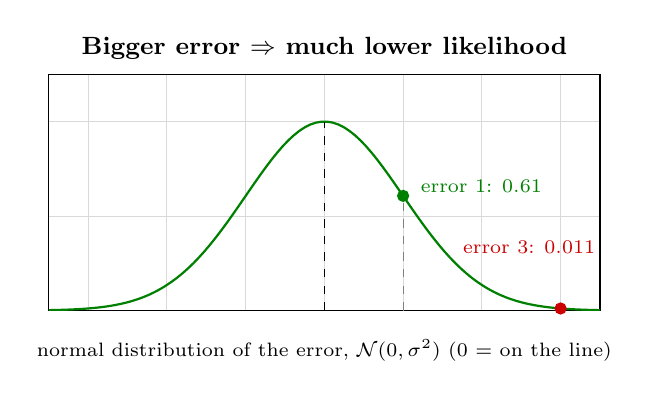
\begin{tikzpicture}
\begin{axis}[scale only axis, width=7cm, height=3cm,
    xmin=-3.5, xmax=3.5, ymin=0, ymax=1.25, enlargelimits=false, grid=major, grid style={gray!30}, major tick length=0pt,
    xticklabels={}, yticklabels={}, title style={yshift=-4pt}, label style={font=\scriptsize},
    title={\small\textbf{Bigger error $\Rightarrow$ much lower likelihood}},
    xlabel={\scriptsize normal distribution of the error, $\mathcal{N}(0, \sigma^2)$ (0 = on the line)}]
\addplot[thick, green!50!black, domain=-3.5:3.5, samples=100] {exp(-x^2/2)};
\addplot[black, dashed] coordinates {(0,0) (0,1)};
\addplot[gray, dashed] coordinates {(1,0) (1,0.607)};
\addplot[only marks, mark=*, green!50!black, mark size=2pt] coordinates {(1,0.607)};
\node[font=\scriptsize, green!50!black, anchor=west] at (axis cs:1.1,0.66) {error 1: $0.61$};
\addplot[only marks, mark=*, red!80!black, mark size=2pt] coordinates {(3,0.011)};
\node[font=\scriptsize, red!80!black, anchor=south] at (axis cs:2.6,0.25) {error 3: $0.011$};
\end{axis}
\end{tikzpicture}
\par}
\end{keeptogether}

\begin{keeptogether}
\textbf{Step 3: Maximize the likelihood.} Maximizing $\ln L(\mathbf{w})$ = minimizing $E(\mathbf{w})$: the constant has no $\mathbf{w}$, and $-\frac{1}{\sigma^2}$ is negative, so maximizing flips into minimizing:
\[
\mathbf{w}_{\text{ML}} = \arg\max_{\mathbf{w}} \ln L(\mathbf{w}) = \arg\min_{\mathbf{w}} E(\mathbf{w})
\]
Picture it with a one-feature line $t = w\,x$, so $w$ is a single number (the slope):

{\centering
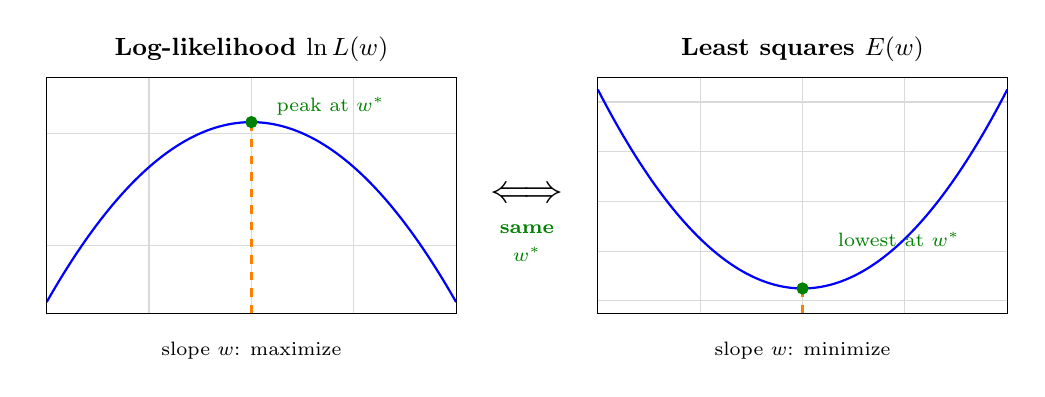
\begin{tikzpicture}
% ---- ln L(w) ----
\begin{axis}[name=lnLw, scale only axis, width=5.2cm, height=3cm,
    xmin=0, xmax=4, ymin=-8, ymax=2.5, enlargelimits=false, grid=major, grid style={gray!30}, major tick length=0pt,
    xticklabels={}, yticklabels={}, title style={yshift=-4pt}, label style={font=\scriptsize},
    title={\small\textbf{Log-likelihood $\ln L(w)$}},
    xlabel={\scriptsize slope $w$: maximize}]
\addplot[thick, blue, domain=0:4, samples=100] {0.5 - 2*(x-2)^2};
\addplot[orange, dashed, thick] coordinates {(2,-8) (2,0.5)};
\addplot[only marks, mark=*, green!50!black, mark size=2pt] coordinates {(2,0.5)};
\node[font=\scriptsize, green!50!black, anchor=west] at (axis cs:2.15,1.2) {peak at $w^*$};
\end{axis}
\node[font=\Large] (eq2) at ([xshift=0.9cm]lnLw.east) {$\Longleftrightarrow$};
\node[font=\scriptsize\bfseries, green!50!black, anchor=north] at ([yshift=-1pt]eq2.south) {same};
\node[font=\scriptsize\bfseries, green!50!black, anchor=north] at ([yshift=-9pt]eq2.south) {$w^*$};
% ---- E(w) ----
\begin{axis}[name=Ew, at={(lnLw.east)}, anchor=west, xshift=1.8cm, scale only axis, width=5.2cm, height=3cm,
    xmin=0, xmax=4, ymin=-0.5, ymax=9, enlargelimits=false, grid=major, grid style={gray!30}, major tick length=0pt,
    xticklabels={}, yticklabels={}, title style={yshift=-4pt}, label style={font=\scriptsize},
    title={\small\textbf{Least squares $E(w)$}},
    xlabel={\scriptsize slope $w$: minimize}]
\addplot[thick, blue, domain=0:4, samples=100] {0.5 + 2*(x-2)^2};
\addplot[orange, dashed, thick] coordinates {(2,-0.5) (2,0.5)};
\addplot[only marks, mark=*, green!50!black, mark size=2pt] coordinates {(2,0.5)};
\node[font=\scriptsize, green!50!black, anchor=south west] at (axis cs:2.25,1.8) {lowest at $w^*$};
\end{axis}
\end{tikzpicture}
\par}
Then set the derivative to 0 and solve:
\[
\nabla_{\mathbf{w}} \ln L(\mathbf{w})
= \frac{1}{\sigma^2}\sum_{n=1}^{N}\big(t_n - \mathbf{w}^\top\mathbf{x}_n\big)\,\mathbf{x}_n = \mathbf{0}
\]
In matrix form ($\sigma^2$ cancels):
\[
\mathbb{X}^\top(\mathbf{t} - \mathbb{X}\mathbf{w}) = \mathbf{0}
\;\Rightarrow\; \mathbb{X}^\top\mathbb{X}\,\mathbf{w} = \mathbb{X}^\top\mathbf{t}
\;\Rightarrow\; \mathbf{w}_{\text{ML}} = (\mathbb{X}^\top\mathbb{X})^{-1}\mathbb{X}^\top\mathbf{t}
\]
That's the normal equation from Linear Regression, so the MLE line \textbf{is} the least-squares line.
\end{keeptogether}

\textbf{Noise model $\Rightarrow$ loss:} Gaussian noise gives squared error. Laplace noise gives absolute error $\sum |t_n - \mathbf{w}^\top\mathbf{x}_n|$, which is less sensitive to outliers.